\documentclass[11pt]{beamer}

\usetheme{Madrid}
\usepackage{amsmath,amssymb}
\usepackage{graphicx}
\usepackage{tikz}
\usepackage[american voltages]{circuitikz}
\usetikzlibrary{decorations.pathreplacing}

% Blank placeholder for a figure that will later be replaced with a real
% circuit diagram (drawio export) or a scan from the source notes.
\newcommand{\blankfig}[3][0.7\linewidth]{%
  \begin{figure}[h!]
    \centering
    \begin{tikzpicture}
      \draw[dashed] (0,0) rectangle (#1,#2);
      \node at (0.5*#1,0.5*#2) {\itshape (figure placeholder)};
    \end{tikzpicture}
    \caption{\small #3}
  \end{figure}
}

\title{Power Electronics --- Chapter 1}
\subtitle{DC-DC Converters: Buck Converter}
\author{POWER\_E\_466}
\date{}

\begin{document}

\frame{\titlepage}

\begin{frame}{Buck Converter}
The buck converter is a DC-DC converter that steps down voltage
($V_{out} < V_{in}$).
\end{frame}

\begin{frame}{Motivating the topology}
Start from a black-box model: given $V_{in} = 50\,\text{V}$, we want an
average output of $V_{out} = 20\,\text{V}$ across a resistive load.

\begin{figure}[h!]
  \centering
  \begin{circuitikz}[scale=0.85, every node/.style={font=\small}]
    \draw (0,0)
      to[V, invert, l=$50\,\mathrm{V}$] (0,3)
      -- (1.5,3);
    \draw (1.5,2.5) rectangle (3.5,3.5);
    \node at (2.5,3) {\Large ?};
    \draw (3.5,3) -- (5,3)
      to[R, l_=$20\,\mathrm{V}$] (5,0)
      -- (0,0);
  \end{circuitikz}
  \caption{\small Black-box step-down converter: $V_{in}=50\,\text{V}$ in, unknown network, $\langle V \rangle = 20\,\text{V}$ across the load.}
\end{figure}
\end{frame}

\begin{frame}{Ideal switch model}
The simplest way to reduce an average voltage is to switch the input on
and off periodically (an ideal SPDT switch connecting the load either to
$V_{in}$ or to ground), so that the average value is controlled by the
fraction of time spent connected to $V_{in}$ --- the \emph{duty cycle}
$D$:
\[
  \langle V \rangle = D \, V_{in}.
\]

\begin{figure}[h!]
  \centering
  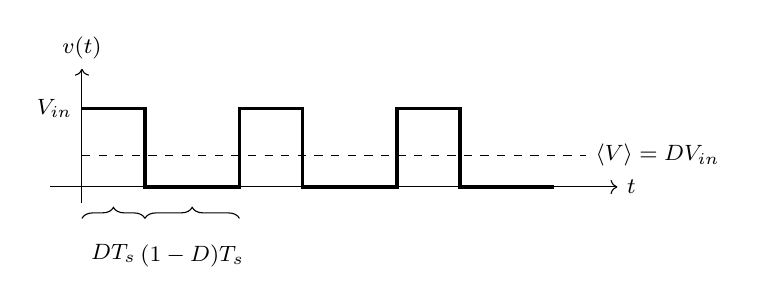
\begin{tikzpicture}[scale=1, every node/.style={font=\footnotesize}]
    \draw[->] (-0.4,0) -- (6.8,0) node[right] {$t$};
    \draw[->] (0,-0.2) -- (0,1.5) node[above] {$v(t)$};
    \draw[very thick]
      (0,1) -- (0.8,1) -- (0.8,0) -- (2,0) -- (2,1) -- (2.8,1) -- (2.8,0)
      -- (4,0) -- (4,1) -- (4.8,1) -- (4.8,0) -- (6,0);
    \node[left] at (0,1) {$V_{in}$};
    \draw[dashed] (0,0.4) -- (6.4,0.4) node[right] {$\langle V\rangle = D V_{in}$};
    \draw[decorate,decoration={brace,amplitude=4pt}] (0,-0.4) -- (0.8,-0.4) node[midway,below=6pt] {$DT_s$};
    \draw[decorate,decoration={brace,amplitude=4pt}] (0.8,-0.4) -- (2,-0.4) node[midway,below=6pt] {$(1-D)T_s$};
  \end{tikzpicture}
  \caption{\small Ideal switch model: pole connects to $V_{in}$ for a
  fraction $D$ of the switching period $T_s$, and to ground for the
  remaining $(1-D)T_s$, producing a PWM waveform whose average is $\langle
  V \rangle$.}
\end{figure}
\end{frame}

\begin{frame}{Why we need an LC filter}
The switched (PWM) waveform is not a clean DC voltage --- it still
contains switching-frequency ripple. From a Fourier-series point of
view, the desired DC output corresponds only to the $f = 0\,\text{Hz}$
(DC offset) term; every other harmonic should be attenuated. A low-pass
\emph{LC filter} does exactly this: it passes the DC component while
suppressing the switching-frequency content.

\begin{figure}[h!]
  \centering
  \begin{circuitikz}[scale=0.65, every node/.style={font=\small}]
    \draw (0,0) to[V, invert, l=$V_{in}$] (0,3) -- (1,3);
    \draw (1,3) circle(0.05);
    \draw (1.05,3) -- (1.8,3.25);
    \draw (2,3) circle(0.05);
    \node[above] at (1.5,3.2) {$D$};
    \draw (2,3) -- (2.7,3) to[L, l=$L$] (4.2,3) -- (5.5,3);
    \draw (5.5,3) to[C, l_=$C$] (5.5,0);
    \draw (5.5,3) -- (7,3) to[R, l_=$R$] (7,0);
    \draw (0,0) -- (7,0);
    \draw (0,0) -- (0,-0.4) node[ground]{};
  \end{circuitikz}
  \caption{\small Buck converter: switch $D$ followed by an $LC$
  low-pass filter, driving a resistive load. This is the buck converter
  topology.}
\end{figure}
\end{frame}

\begin{frame}{Inductor and capacitor averaging identities}
For an inductor,
\[
  v = L \frac{di}{dt}
  \quad\Longleftrightarrow\quad
  i = \frac{1}{L}\int v \, dt,
\]
so if $i$ is periodic in steady state, the average inductor voltage must
be zero:
\[
  \langle v_L \rangle = 0 \qquad \text{(volt-second balance)}.
\]

For a capacitor,
\[
  i = C \frac{dv}{dt}
  \quad\Longleftrightarrow\quad
  v = \frac{1}{C}\int i \, dt,
\]
so if $v$ is periodic in steady state, the average capacitor current
must be zero:
\[
  \langle i_C \rangle = 0 \qquad \text{(current-second/charge balance)}.
\]
\end{frame}

\begin{frame}{Steady-state inductor current ripple}
Over one switching period $T_s$, the inductor current $i_L$ ramps up
while the switch connects to $V_{in}$ (duration $DT_s$) and ramps down
while it connects to ground (duration $(1-D)T_s$):
\[
  \frac{di_L}{dt} = \frac{v_L}{L}, \qquad
  2\,\Delta i_L = \frac{V}{L}\,D T_s
  \quad\text{(rising)}, \qquad
  2\,\Delta i_L = \frac{V}{L}\,(1-D) T_s
  \quad\text{(falling)}.
\]

\begin{figure}[h!]
  \centering
  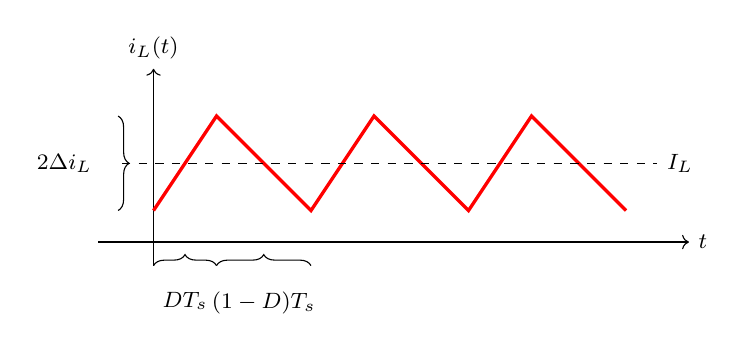
\begin{tikzpicture}[scale=1, every node/.style={font=\footnotesize}]
    \draw[->] (-0.7,0) -- (6.8,0) node[right] {$t$};
    \draw[->] (0,-0.3) -- (0,2.2) node[above] {$i_L(t)$};
    \draw[very thick,red]
      (0,0.4) -- (0.8,1.6) -- (2,0.4) -- (2.8,1.6) -- (4,0.4) -- (4.8,1.6) -- (6,0.4);
    \draw[dashed] (-0.4,1) -- (6.4,1) node[right] {$I_L$};
    \draw[decorate,decoration={brace,amplitude=4pt,mirror}] (-0.45,0.4) -- (-0.45,1.6) node[midway,left=6pt] {$2\Delta i_L$};
    \draw[decorate,decoration={brace,amplitude=4pt}] (0,-0.3) -- (0.8,-0.3) node[midway,below=6pt] {$DT_s$};
    \draw[decorate,decoration={brace,amplitude=4pt}] (0.8,-0.3) -- (2,-0.3) node[midway,below=6pt] {$(1-D)T_s$};
  \end{tikzpicture}
  \caption{\small Steady-state inductor current: triangular ripple of
  peak-to-peak $2\Delta i_L$, rising for $DT_s$ and falling for
  $(1-D)T_s$ each switching period.}
\end{figure}
\end{frame}

\begin{frame}{Worked example: switch ON}
Given $V_{in} = 50\,\text{V}$, $D = 0.5$, $L = 10\,\text{mH}$,
$T_s = 1\,\text{ms}$, and (for this simplified example) an output branch
modelled as a current source with $V = 0$:

\[
  \frac{di_L}{dt} = \frac{50}{10^{-3}} = 50\times10^{3}\ \text{A/s}
  \;\longrightarrow\; \Delta i_L = 5\,\text{A}.
\]
At $t=0^+$: $i_L = 5\,\text{A}$, $i_O = 0$, $i_C = i_L - i_O = 5\,\text{A}$.

\begin{figure}[h!]
  \centering
  \begin{circuitikz}[scale=0.75, every node/.style={font=\small}]
    \draw (0,0) to[V, invert, l=$50\,\mathrm{V}$] (0,3) -- (1,3);
    \draw (1,3) circle(0.05) -- (2,3) circle(0.05);
    \node[above] at (1.5,3.15) {$D$ (closed)};
    \draw (2,3) -- (2.6,3) to[L, l=$10\,\mathrm{mH}$] (4.3,3) -- (5.2,3);
    \draw (5.2,2.5) rectangle (6.6,3.5);
    \node at (5.9,3) {$V=0$};
    \draw (5.2,2.5) -- (5.2,0) -- (0,0);
    \draw (0,0) -- (0,-0.4) node[ground]{};
  \end{circuitikz}
  \caption{\small Buck circuit during the ON interval: $V_{in}=50\,\text{V}$, $D=0.5$, $L=10\,\text{mH}$, $T_s=1\,\text{ms}$, output branch at $V=0$.}
\end{figure}
\end{frame}

\begin{frame}{Worked example: switch OFF}
\[
  \frac{di_L}{dt} = \frac{0}{10^{-3}} = 0\ \text{A/s},
\]
so $i_L$ stays constant at $5\,\text{A}$ while the switch is off (for
this particular example, since the inductor sees $0\,\text{V}$ in both
states here).

\begin{figure}[h!]
  \centering
  \begin{circuitikz}[scale=0.75, every node/.style={font=\small}]
    \draw (0,0) to[V, invert, l=$50\,\mathrm{V}$] (0,3) -- (1,3);
    \draw (1,3) circle(0.05);
    \draw (1.05,3) -- (1.6,3.3);
    \draw (2,3) circle(0.05);
    \node[above] at (1.5,3.35) {$D$ (open)};
    \draw (2,3) -- (2.6,3) to[L, l=$10\,\mathrm{mH}$] (4.3,3) -- (5.2,3);
    \draw (5.2,2.5) rectangle (6.6,3.5);
    \node at (5.9,3) {$V=0$};
    \draw (5.2,2.5) -- (5.2,0) -- (0,0);
    \draw (0,0) -- (0,-0.4) node[ground]{};
  \end{circuitikz}
  \caption{\small Buck circuit during the OFF interval, same
  component values as above.}
\end{figure}
\end{frame}

\begin{frame}{Is this steady state?}
Not necessarily --- $V_{out}$ can still change from cycle to cycle if
the circuit is not yet in continuous, periodic operation. As $i_O$
increases from $0$, $i_C = i_L - i_O$ decreases; by charge balance,
$\langle i_C \rangle = 0$ is exactly the condition that defines the
steady-state operating point.

\begin{figure}[h!]
  \centering
  \begin{circuitikz}[scale=0.75, every node/.style={font=\small}]
    \draw (0,0) to[V, invert, l=$50\,\mathrm{V}$] (0,3) -- (1,3);
    \draw (1,3) circle(0.05) -- (2,3) circle(0.05);
    \node[above] at (1.5,3.15) {$D$};
    \draw (2,3) -- (2.6,3) to[L, l=$10\,\mathrm{mH}$] (4.3,3) -- (5.2,3);
    \draw (5.2,2.5) rectangle (6.6,3.5);
    \node at (5.9,3) {$V=2.5$};
    \draw[->,thick] (6.9,3.6) -- (6.9,4.1) node[above]{$i_O\!\uparrow$};
    \draw (5.2,2.5) -- (5.2,0) -- (0,0);
    \draw (0,0) -- (0,-0.4) node[ground]{};
  \end{circuitikz}
  \caption{\small Buck circuit with increased output current
  ($V \approx 2.5\,\text{V}$ example): as $i_O \uparrow$, $i_C \downarrow$,
  illustrating the approach to $\langle i_C \rangle = 0$ (charge balance).}
\end{figure}
\end{frame}

\begin{frame}{Approaching steady state}
\begin{figure}[h!]
  \centering
  \begin{tikzpicture}[scale=0.85, every node/.style={font=\scriptsize}]
    \draw[->] (-0.3,0) -- (8.5,0) node[right] {$t$};
    \draw[->] (0,-0.3) -- (0,4) node[above] {$i_L(t)$};
    \draw[very thick]
      (0,0) -- (0.4,1.4) -- (1,1.0)
      -- (1.4,2.1) -- (2,1.7)
      -- (2.4,2.6) -- (3,2.3)
      -- (3.4,3.0) -- (4,2.75);
    \node at (5,2.9) {$\cdots$};
    \draw[very thick]
      (6,2.75) -- (6.4,3.3) -- (7,3.05)
      -- (7.4,3.35) -- (8,3.1);
    \node[left] at (-0.1,0) {$i_L(0)=0$};
    \draw[dashed] (0.4,0) -- (0.4,1.4); \node[below] at (0.4,-0.05) {$DT_s$};
    \draw[dashed] (2,0) -- (2,1.7); \node[below] at (2,-0.05) {$2T_s$};
    \draw[dashed] (7,0) -- (7,3.05); \node[below] at (7,0) {$nT_s$};
    \draw[dashed] (8,0) -- (8,3.1); \node[below] at (8,0) {$(n{+}1)T_s$};
  \end{tikzpicture}
  \caption{\small Classic multi-period inductor current waveform
  $i_L(t)$ ramping toward steady state: slope $\frac{V_g - v(t)}{L}$
  while on, slope $\frac{-v(t)}{L}$ while off, converging so that
  $i_C \approx 0$ in steady state (cf.\ Erickson, \emph{Fundamentals of
  Power Electronics}).}
\end{figure}
\end{frame}

\begin{frame}{Realizing the switch with real devices}
The ideal SPDT switch (poles $A$, $B$, $C$) is not a physical component.
It is realized using one \emph{active} switch (a transistor, controlled
by a gate/base signal) for the $A$--$B$ throw, and one \emph{passive}
switch (a diode, which conducts automatically depending on the
circuit's own voltage/current) for the $C$--$B$ throw.

\begin{figure}[h!]
  \centering
  \begin{circuitikz}[scale=0.75, every node/.style={font=\small}]
    \draw (0,0) to[V, invert, l=$V_{S}$] (0,3) -- (1,3);
    \draw (1,2.6) rectangle (2.4,3.4);
    \node at (1.7,3) {MOSFET};
    \node[above] at (1,3.4) {$A$};
    \node[above] at (2.4,3.4) {$B$};
    \draw (2.4,3) -- (3.2,3);
    \draw (3.2,3) -- (3.2,2.2);
    \draw[fill=black] (3.0,2.2) -- (3.4,2.2) -- (3.2,1.7) -- cycle;
    \draw (3.0,1.7) -- (3.4,1.7);
    \draw (3.2,1.7) -- (3.2,0);
    \node[right] at (3.5,1.95) {diode ($C$--$B$)};
    \draw (3.2,3) -- (3.9,3) to[L, l=$L$] (5.4,3) -- (6.2,3);
    \draw (6.2,3) to[C, l_=$C$] (6.2,0);
    \draw (6.2,3) -- (7.6,3) to[R, l_=$R$] (7.6,0);
    \draw (0,0) -- (7.6,0);
    \draw (0,0) -- (0,-0.4) node[ground]{};
  \end{circuitikz}
  \caption{\small Replacing the ideal switch with a MOSFET (A--B)
  and a diode (C--B), giving the practical buck converter realization.}
\end{figure}
\end{frame}

\begin{frame}{Switch analysis: node A--B (transistor position)}
When the ideal switch is ON: $V_{AB} = 0$, $I_{AB} = I_L$. When OFF:
$V_{AB} = V_S$, $I_{AB} = 0$. This $(I,V)$ locus (first quadrant only:
on along the current axis, off along the voltage axis) matches an
\emph{active} switch such as a MOSFET/BJT/IGBT.

\begin{figure}[h!]
  \centering
  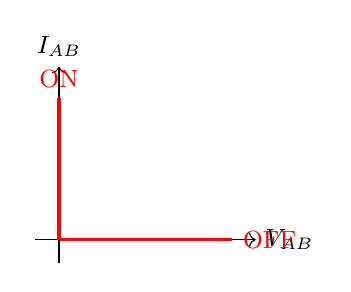
\begin{tikzpicture}[scale=1,every node/.style={font=\small}]
    \draw[->] (-0.3,0) -- (2.5,0) node[right] {$V_{AB}$};
    \draw[->] (0,-0.3) -- (0,2.2) node[above] {$I_{AB}$};
    \draw[very thick,red] (0,0) -- (0,1.8) node[above]{ON};
    \draw[very thick,red] (0,0) -- (2.2,0) node[right]{OFF};
  \end{tikzpicture}
  \caption{\small $I_{AB}$--$V_{AB}$ switch locus for the transistor
  position: ON along the current axis, OFF along the voltage axis.}
\end{figure}
\end{frame}

\begin{frame}{Switch analysis: node C--B (diode position)}
When the ideal switch is ON (meaning the $A$--$B$ throw is closed):
$V_{CB} = -V_S$, $I_{CB} = 0$. When OFF (meaning $C$--$B$ conducts
instead): $V_{CB} = 0$, $I_{CB} = I_L$. This locus (blocks negative
voltage, conducts positive current, no external control terminal)
matches a \emph{passive} switch: a diode.

\begin{figure}[h!]
  \centering
  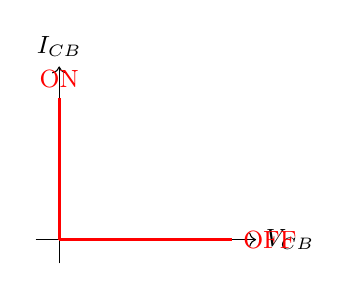
\begin{tikzpicture}[scale=1,every node/.style={font=\small}]
    \draw[->] (-0.3,0) -- (2.5,0) node[right] {$V_{CB}$};
    \draw[->] (0,-0.3) -- (0,2.2) node[above] {$I_{CB}$};
    \draw[very thick,red] (0,0) -- (0,1.8) node[above]{ON};
    \draw[very thick,red] (0,0) -- (2.2,0) node[right]{OFF};
  \end{tikzpicture}
  \caption{\small $I_{CB}$--$V_{CB}$ switch locus for the diode
  position: blocks reverse voltage, conducts forward current.}
\end{figure}
\end{frame}

\begin{frame}{Switch device characteristics}
\begin{itemize}
  \item \textbf{BJT / IGBT} are active switches: the conducting state is
  set entirely by the control-terminal signal, independent of the
  waveforms at the power terminals. Ideal characteristic: $i = 0$ when
  off (blocks $v \geq 0$); $v \approx 0$ when on (conducts
  $i \geq 0$). Poor/no reverse-conducting or reverse-blocking
  capability.
  \item \textbf{MOSFET} behaves similarly, but can additionally conduct
  in reverse. It is normally operated with $i \geq 0$, same as BJT/IGBT,
  so an active SPST switch can be realized with a BJT, IGBT, or MOSFET.
  \item \textbf{Diode} is a passive switch with no control terminal: its
  state is determined entirely by the terminal waveforms $i(t)$,
  $v(t)$. Ideal characteristic: off ($i=0$) when $v<0$; on ($v=0$) when
  $i>0$. It can block negative voltage but not positive voltage.
\end{itemize}
\end{frame}

\begin{frame}{Switch device characteristics (reference figures)}
\begin{figure}[h!]
  \centering
  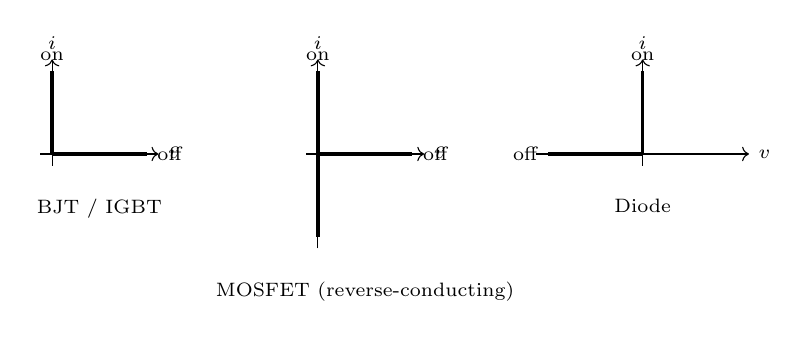
\begin{tikzpicture}[scale=0.75, every node/.style={font=\scriptsize}]
    \begin{scope}
      \draw[->] (-0.2,0) -- (1.8,0) node[right]{$v$};
      \draw[->] (0,-0.2) -- (0,1.6) node[above]{$i$};
      \draw[very thick] (0,0) -- (0,1.4) node[above]{on};
      \draw[very thick] (0,0) -- (1.6,0) node[right]{off};
      \node[below] at (0.8,-0.6) {BJT / IGBT};
    \end{scope}
    \begin{scope}[xshift=4.5cm]
      \draw[->] (-0.2,0) -- (1.8,0) node[right]{$v$};
      \draw[->] (0,-1.6) -- (0,1.6) node[above]{$i$};
      \draw[very thick] (0,-1.4) -- (0,1.4) node[above]{on};
      \draw[very thick] (0,0) -- (1.6,0) node[right]{off};
      \node[below] at (0.8,-2) {MOSFET (reverse-conducting)};
    \end{scope}
    \begin{scope}[xshift=10cm]
      \draw[->] (-1.8,0) -- (1.8,0) node[right]{$v$};
      \draw[->] (0,-0.2) -- (0,1.6) node[above]{$i$};
      \draw[very thick] (0,0) -- (0,1.4) node[above]{on};
      \draw[very thick] (0,0) -- (-1.6,0) node[left]{off};
      \node[below] at (0,-0.6) {Diode};
    \end{scope}
  \end{tikzpicture}
  \caption{\small Idealized switch characteristics for BJT/IGBT, MOSFET,
  and diode (simplified from the textbook reference figures --- the
  real-world $I$-$V$ curve families are omitted here).}
\end{figure}
\end{frame}

\begin{frame}{Buck: Summary}
\begin{figure}[h!]
  \centering
  \begin{circuitikz}[scale=0.75, every node/.style={font=\small}]
    \draw (0,0) to[V, invert, l=$V_{S}$] (0,3) -- (1,3);
    \draw (1,2.6) rectangle (2.4,3.4);
    \node at (1.7,3) {MOSFET};
    \node[above] at (1,3.4) {$A$};
    \node[above] at (2.4,3.4) {$B$};
    \draw (2.4,3) -- (3.2,3);
    \draw (3.2,3) -- (3.2,2.2);
    \draw[fill=black] (3.0,2.2) -- (3.4,2.2) -- (3.2,1.7) -- cycle;
    \draw (3.0,1.7) -- (3.4,1.7);
    \draw (3.2,1.7) -- (3.2,0);
    \node[right] at (3.5,1.95) {diode ($C$--$B$)};
    \draw (3.2,3) -- (3.9,3) to[L, l=$L$] (5.4,3) -- (6.2,3);
    \draw (6.2,3) to[C, l_=$C$] (6.2,0);
    \draw (6.2,3) -- (7.6,3) to[R, l_=$R$] (7.6,0) node[right, xshift=6pt]{$V_O$};
    \draw (0,0) -- (7.6,0);
    \draw (0,0) -- (0,-0.4) node[ground]{};
  \end{circuitikz}
  \caption{\small Final buck converter circuit: MOSFET (A--B),
  freewheeling diode (C--B), $LC$ output filter, load.}
\end{figure}

\[
  \boxed{V_O = D\,V_S}
  \qquad\text{with } \langle i_C \rangle \to 0 \text{ in steady state.}
\]
\end{frame}

\end{document}
